%!TEX root = /Users/jakubkonka/Thesis/Thesis.tex
\chapter{Static Analysis of Network Selection Mechanism: Indirect Approach}
\label{cha:indirect}

\minitoc
\vspace{10mm}

In this chapter, the bidding problem described in Section~\ref{sec:problem_definition_and_assumptions_direct} will be transformed from a bidding problem with symmetric type (or cost) distributions into a bidding problem with asymmetric type distributions. This type of bidding problems has already been researched by the economic community, both in a very specific setting (two bidders, specific type distributions) \cite{KaplanZamir2007,MaskinRiley2000}, and in a very general setting ($n$ bidders, arbitrary type distributions) \cite{Lebrun1999,Lebrun2006}, and hence there exist results that are applicable to the problem at hand.

In order to transform the problem, recall the utility function for each network operator $i$
\begin{equation*}
  u_i(b,c,r) = \left\{
  \begin{array}{l l}
    b_i-c_i & \;\text{if } wb_i + (1-w)r_i < \displaystyle\min_{j\neq i}[wb_j + (1-w)r_j],\\
    0 & \;\text{if } wb_i + (1-w)r_i > \displaystyle\min_{j\neq i}[wb_j + (1-w)r_j],
  \end{array}\right.
\end{equation*}
and let
\begin{equation}
  \label{eq:b_hat_indirect}
  \hat{b}_i = wb_i + (1-w)r_i \quad\text{for all } i\in N.
\end{equation}
(Note that the new bid is just an alias for the compound bid, and in fact, they are equivalent; $\beta(b_i,r_i)\equiv\hat{b}_i$.) Solving Equation~\eqref{eq:b_hat_indirect} for $b_i$ yields
\begin{equation}
  \label{eq:b_from_b_hat_indirect}
  b_i = \frac{\hat{b}_i - (1-w)r_i}{w}, \quad w\neq 0.
\end{equation}
Substituting Equation~\eqref{eq:b_from_b_hat_indirect} back into the utility function yields
\begin{equation*}
  u_i(\hat{b},c,r) = \left\{
  \begin{array}{l l}
    \displaystyle\frac{1}{w}\left[\hat{b}_i-(wc_i + (1-w)r_i)\right] & \;\text{if } \hat{b}_i < \displaystyle\min_{j\neq i}\hat{b}_j,\\[2ex]
    0 & \;\text{if } \hat{b}_i > \displaystyle\min_{j\neq i}\hat{b}_j.
  \end{array}\right.
\end{equation*}
If we further let
\begin{equation}
  \label{eq:cost_hat_indirect}
  \hat{c}_i = wc_i + (1-w)r_i \quad\text{for all } i\in N,
\end{equation}
the utility function simplifies to
\begin{equation}
  \label{eq:sellers_utility_hat_indirect}
  u_i(\hat{b},\hat{c}) = \left\{
  \begin{array}{l l}
    \displaystyle\frac{1}{w}\left(\hat{b}_i-\hat{c}_i\right) & \;\text{if } \hat{b}_i < \displaystyle\min_{j\neq i}\hat{b}_j,\\[2ex]
    0 & \;\text{if } \hat{b}_i > \displaystyle\min_{j\neq i}\hat{b}_j.
  \end{array}\right.
\end{equation}
In order to avoid ambiguity, we shall refer to $\hat{c}_i$ as costs-hat and $\hat{b}_i$ as bids-hat, while still referring to $c_i$ as costs and $b_i$ as bids. Note, moreover, that since both $w$ and $r_i$ are assumed to be given to the network operators (i.e., they cannot directly modify their values), the costs-hat and bids-hat are simply convex (and hence, linear) combinations involving costs and bids respectively (Equations~\eqref{eq:b_hat_indirect}~and~\eqref{eq:cost_hat_indirect}). Therefore, a network operator bidding their cost-hat is equivalent to bidding their cost.

As a result of this transformation, the costs-hat, $\hat{c}_i$, for each network operator $i$ are distributed over the interval
\begin{equation*}
  \hat{c}_i\in [(1-w)r_i, (1-w)r_i + w]\equiv [\underline{\hat{c}}_i, \bar{\hat{c}}_i]
\end{equation*}
since $c_i\in [0,1]$ for all $i\in N$. Note, moreover, that for all $i\in N$
\begin{equation*}
  [\underline{\hat{c}}_i, \bar{\hat{c}}_i] \subset [0,1]
\end{equation*}
since $w\in (0,1)$ and $r_i\in [0,1]$, and in particular, if $w=1$
\begin{equation*}
  [\underline{\hat{c}}_i, \bar{\hat{c}}_i] = [0,1].
\end{equation*}
Therefore, in terms of costs-hat, the network operators are \emph{ex ante} asymmetric; that is, due to differing domains of costs-hat between the network operators, the probability distributions will have differing supports.

With these results at hand, we can proceed with the analysis of the auction.

\section{Generic Case} % (fold)
\label{sec:generic_case_indirect}
In the generic case, with arbitrary probability distributions of costs and $n\ge 2$ network operators, recall that: if $w=0$, then Proposition~\ref{prop:special_case_w_0_direct} holds; if $w=1$, then Proposition~\ref{prop:special_case_w_1_direct} holds; and if $r_i=r_j$ for all $i,j\in N$ such that $i\neq j$, then Corollary~\ref{cor:special_case_r_i_r_j_direct} holds. Therefore, it suffices to consider only the case when $w\in (0,1)$.

Firstly, note that under the generic assumptions specified in Section~\ref{sec:problem_definition_and_assumptions_direct} and $w\in (0,1]$, the problem satisfies the following regularity conditions.
\begin{proposition}[Regularity Conditions]
\label{prop:regularity_conditions_indirect}
Let $F_i$ be the distribution function of $\hat{c}_i$ for all $i\in N$, and suppose $w\in (0,1]$. Then,
\begin{enumerate}
  \item the support of $F_i$ is an interval ${[\underline{\hat{c}}_i, \bar{\hat{c}}_i]}$;
  \item $F_i$ is differentiable over ${(\underline{\hat{c}}_i, \bar{\hat{c}}_i]}$ with a derivative $f_i$ locally bounded away from zero over this interval; and
  \item $F_i$ is atomless.
\end{enumerate}
\end{proposition}
The regularity conditions in Proposition~\ref{prop:regularity_conditions_indirect} correspond to the regularity assumptions on type distributions put forward by Lebrun~\cite{Lebrun2006} (cf. Assumptions~A.1 in~\cite{Lebrun2006}). Therefore, since our problem satisfies Lebrun's assumptions, his results are applicable to our problem.

We further assume that
\begin{assumptions}
\label{ass:assumptions_generic_indirect}
Assume that
\begin{enumerate}
  \item $w\in(0,1)$;
  \item there exists $i\in N$ such that $r_i\neq r_j$ for all $i\neq j$ and $j\in N$; and
  \item without loss of generality, let network operator 1 be characterized by the lowest reputation rating; that is, $r_1 \leq r_i$ for all $i\in N$ such that $i\neq 1$. If there exists $j\in N$ such that $j\neq 1$ and $r_1 = r_j$, then we make an additional assumption that there exists $\delta > 0$ such that $F_i$ is strictly log-concave over $(\bar{\hat{c}}_1 - \delta, \bar{\hat{c}}_1)\cap (\underline{\hat{c}}_i, \bar{\hat{c}}_i)$ for all $i\in N$.
\end{enumerate}
\end{assumptions}

In equilibrium, the bids of each network operator equal $\hat{b}_i = \hat{b}_i(\hat{c}_i)$, where $\hat{b}_i$ is the equilibrium bidding function. Denote by $\hat{c}_i(\hat{b}_i)\equiv \hat{b}_i^{-1}(\hat{b}_i)$ an inverse equilibrium bidding function for each network operator $i\in N$. Therefore, the expected utility for each network operator $i\in N$ can be written as
\begin{align*}
  \Pi_i(\hat{b}_i,\hat{c}_i,\hat{b}_{-i},\hat{c}_{-i})
  &\equiv (\hat{b}_i - \hat{c}_i)P\{\text{winning}\mid\hat{b}_i\}\\
  &= (\hat{b}_i - \hat{c}_i)Q_i(\hat{b}_i),
\end{align*}
where
\begin{equation*}
Q_i(\hat{b}_i) = \prod_{j\neq i}\left( 1 - F_j(\hat{c}_j(\hat{b}_i)) \right)
\end{equation*}
is the probability that network operator $i$ is the lowest bidder.

The first order condition for maximizing network operator $i$'s expected utility is
\begin{equation}
  \label{eq:foc_indirect}
  \frac{d}{d\hat{b}_i}\Pi_i(\hat{b}_i,\hat{c}_i,\hat{b}_{-i},\hat{c}_{-i}) = Q_i(\hat{b}_i) + (\hat{b}_i - \hat{c}_i)\cdot\frac{d}{d\hat{b}_i}Q_i(\hat{b}_i) = 0,
\end{equation}
where
\begin{equation*}
  \frac{d}{d\hat{b}_i}Q_i(\hat{b}_i) = (-1)\sum_{j\neq i} f_j(\hat{c}_j(\hat{b}_i))\frac{d}{d\hat{b}_i}\hat{c}_j(\hat{b}_i)\prod_{k\neq j} \left( 1 - F_k(\hat{c}_k(\hat{b}_i)) \right).
\end{equation*}

Noting that in equilibrium $\hat{c}_i = \hat{c}_i(\hat{b}_i)$, letting $\hat{b}_i = b$, and rearranging terms in Equation~\eqref{eq:foc_indirect} yields
\begin{align}
  \label{eq:foc_simplified_indirect}
  \frac{1}{b - \hat{c}_i(b)} 
  &= \frac{\sum_{j\neq i} f_j(\hat{c}_j(b))\frac{d}{db}\hat{c}_j(b)\prod_{k\neq j} \left( 1 - F_k(\hat{c}_k(b)) \right)}{\prod_{j\neq i} \left( 1 - F_j(\hat{c}_j(b)) \right)}\nonumber \\[2ex]
  &= \sum_{j\neq i}\frac{f_j(\hat{c}_j(b))}{1 - F_j(\hat{c}_j(b))}\cdot\frac{d}{db}\hat{c}_j(b).
\end{align}
Summing Equation~\eqref{eq:foc_simplified_indirect} over all $n$ network operators yields
\begin{equation}
  \label{eq:foc_summed_indirect}
  \frac{1}{n-1}\sum_{i=1}^n \frac{1}{b - \hat{c}_i(b)} = \sum_{i=1}^n \frac{f_i(\hat{c}_i(b))}{1 - F_i(\hat{c}_i(b))}\cdot\frac{d}{db}\hat{c}_i(b).
\end{equation}
Subtracting Equation~\eqref{eq:foc_simplified_indirect} from \eqref{eq:foc_summed_indirect} yields 
\begin{equation*}
  \frac{1}{n-1}\sum_{i=1}^n \frac{1}{b - \hat{c}_i(b)} - \frac{1}{b - \hat{c}_i(b)} = \frac{f_i(\hat{c}_i(b))}{1 - F_i(\hat{c}_i(b))}\cdot\frac{d}{db}\hat{c}_i(b)
\end{equation*}
which leads to the system of nonlinear ordinary differential equations (ODE)
\begin{equation*}
  \frac{d}{db}\hat{c}_i(b) = \frac{1 - F_i(\hat{c}_i(b))}{f_i(\hat{c}_i(b))}\left[ \frac{1}{n-1}\sum_{i=1}^n \frac{1}{b-\hat{c}_i(b)} - \frac{1}{b-\hat{c}_i(b)} \right]
\end{equation*}
for $i=1,2,\dotsc,n$. As we shall see briefly, there exists a unique set of inverse bidding functions that satisfy the system and constitute a pure-strategy Bayesian Nash equilibrium where network operators submit at least their costs-hat. Firstly, we need to define a few concepts (cf.~Definitions 1, 2 and 3 in Lebrun~\cite{Lebrun2006}).

\begin{define}[Upper bound on bids]
\label{def:upper_bound_bids_indirect}
Let Assumptions~\ref{ass:assumptions_generic_indirect} be satisfied. Then, the upper bound on bids is defined as follows
\begin{equation}
  \label{eq:upper_bound_bids_indirect}
  \bar{\hat{b}} = \min\arg\max_{b\in[\bar{\hat{c}}_1, \bar{\hat{c}}_2]}(b - \bar{\hat{c}}_1)\prod_{i>1}\left( 1 - F_i(b) \right).
\end{equation}
\end{define}

\begin{define}[Feasible bidders]
\label{def:feasible_bidders_indirect}
Let Assumptions~\ref{ass:assumptions_generic_indirect} be satisfied. Let $J$ denote the set of feasible bidders. Then, $J$ is a subset of $N$ such that
\begin{equation*}
  J = \left\{j \:\middle\vert\: 1\leq j\leq n \text{ and } \underline{\hat{c}}_j < \bar{\hat{b}}\right\}.
\end{equation*}
Further let $n' = |J|$.
\end{define}

\begin{define}[Characterization of lower bound on bids]
\label{def:lower_bound_bids_indirect}
Let Assumptions~\ref{ass:assumptions_generic_indirect} be satisfied. Then,
\begin{enumerate}
  \item For all $\underline{\hat{b}}\in (\underline{\hat{c}}_2, \bar{\hat{b}})$, there exists one and only one\footnote{See Lemma A4.1, Appendix 4 in Lebrun~\cite{Lebrun2004} for proof.} $k(\underline{\hat{b}})\in \{2,\dotsc,n\}$ such that $\underline{\hat{c}}_{k(\underline{\hat{b}})} < \underline{\hat{b}}$ and
  \begin{equation*}
    \frac{1}{\underline{\hat{b}} - \underline{\hat{c}}_{k(\underline{\hat{b}})}}\leq \frac{1}{k(\underline{\hat{b}}) - 1}\sum_{i=1}^{k(\underline{\hat{b}})}\frac{1}{\underline{\hat{b}} - \underline{\hat{c}}_i},
  \end{equation*}
  and if $\underline{\hat{c}}_{k(\underline{\hat{b}})+1} < \underline{\hat{b}}$ (and $k(\underline{\hat{b}}) < n$)
  \begin{equation*}
    \frac{1}{k(\underline{\hat{b}}) - 1}\sum_{i=1}^{k(\underline{\hat{b}})}\frac{1}{\underline{\hat{b}} - \underline{\hat{c}}_i} < \frac{1}{\underline{\hat{b}} - \underline{\hat{c}}_{k(\underline{\hat{b}})+1}}.
  \end{equation*}
  \item For all $\underline{\hat{b}}\in (\underline{\hat{c}}_2, \bar{\hat{b}})$, let $\hat{c}(\underline{\hat{b}})$ be defined as follows
  \begin{equation}
  \label{eq:lower_bound_bids_cost_indirect}
    \hat{c}(\underline{\hat{b}}) = \underline{\hat{b}} - \sfrac{\left(k(\underline{\hat{b}})-1\right)}{\left(\sum_{i=1}^{k(\underline{\hat{b}})} \frac{1}{\underline{\hat{b}} - \underline{\hat{c}}_i}\right)}.
  \end{equation}
\end{enumerate}
\end{define}
\noindent Note that Definition~\ref{def:lower_bound_bids_indirect} implies
\begin{equation}
  \label{eq:bounds_lower_bound_bids_cost_indirect}
  \begin{array}{lll}
    &\underline{\hat{c}}_{k(\underline{\hat{b}})} \leq \hat{c}(\underline{\hat{b}}) < \underline{\hat{c}}_{k(\underline{\hat{b}})+1} &\text{if}\quad k(\underline{\hat{b}}) < n,\\
    \text{and } 
    &\underline{\hat{c}}_{k(\underline{\hat{b}})} \leq \hat{c}(\underline{\hat{b}}) &\text{if}\quad k(\underline{\hat{b}}) = n.
  \end{array}
\end{equation}

With those definitions at hand, we can proceed with the characterization of the equilibrium which is due to Lebrun~\cite{Lebrun2006}.
\begin{proposition}[Characterization of the Equilibrium]
\label{prop:characterization_of_the_equilibrium_indirect}
Let Assumptions~\ref{ass:assumptions_generic_indirect} be satisfied. There exists one and only one pure-strategy Bayesian Nash equilibrium where network operators submit at least their costs-hat. In every such equilibrium, network operator $i\in J$ follows a bid function $\hat{b}_i$, for all $1\leq i\leq n$. Moreover, there exists $\underline{\hat{b}}\in (\underline{\hat{c}}_2, \bar{\hat{b}})$ such that, for all $i\in J$, there exists a continuous extension of $\hat{b}_i$ to the interval $\left[\min\{\underline{\hat{c}}_i, \hat{c}(\underline{\hat{b}})\}, \bar{\hat{b}}\right]$ that is differentiable with a strictly positive derivative everywhere over this interval, except possibly at $\underline{\hat{c}}_i$ or when its value is equal to $\bar{\hat{b}}$, and such that the inverse bid functions $\hat{c}_i$ for all $i\in J$ of these extensions, where differentiable, satisfy the following system of differential equations
\begin{equation}
  \label{eq:foc_ode_indirect}
  \frac{d}{db}\hat{c}_i(b) = \frac{1 - F_i(\hat{c}_i(b))}{f_i(\hat{c}_i(b))}\left[ \frac{1}{n-1}\sum_{k=1}^n \frac{1}{b-\hat{c}_k(b)} - \frac{1}{b-\hat{c}_i(b)} \right]
\end{equation}
for all $1\leq i\leq n$, with the following lower boundary condition
\begin{equation}
  \label{eq:foc_ode_lower_boundary_indirect}
  \hat{c}_i(\underline{\hat{b}}) = \min\left\{\underline{\hat{c}}_i, \hat{c}(\underline{\hat{b}})\right\} \quad\text{for all }i\in J
\end{equation}
and the upper boundary condition
\begin{equation}
  \label{eq:foc_ode_upper_boundary_indirect}
  \hat{c}_i(\bar{\hat{b}}) = \bar{\hat{b}}
\end{equation}
for all, except possibly one, $1\leq i\leq n$.
\end{proposition}
The intuition behind the upper boundary condition in Equation~\eqref{eq:foc_ode_upper_boundary_indirect} is that the network operator bids their cost-hat when their probability of winning is zero. Ignoring the minimum operator, the intuition behind the lower boundary condition in Equation~\eqref{eq:foc_ode_lower_boundary_indirect} on the other hand, is that the lowest bid-hat of each network operator is reached for their lowest cost-hat.

Since both $w$ and $r_i$ are assumed to be given to the network operators (i.e., they cannot directly modify their values), the costs-hat and bids-hat are simply convex (and hence, linear) combinations involving costs and bids respectively (Equations~\eqref{eq:b_hat_indirect}~and~\eqref{eq:cost_hat_indirect}). Therefore, a network operator bidding their cost-hat is equivalent to bidding their cost, and we immediately deduce the following corollary.
\begin{corollary}
\label{cor:characterization_of_the_equilibrium}
Let Assumptions~\ref{ass:assumptions_generic_indirect} be satisfied. There exists one and only one pure-strategy Bayesian Nash equilibrium where network operators submit at least their costs.
\end{corollary}

Even though we are guaranteed that there exists a unique equilibrium to our problem, the establishment of a closed-form solution to the system of ODEs for $n\ge 2$ network operators and arbitrary cost distribution is very difficult (if possible), and for $n>2$ is not possible \cite{Lebrun2006, Krishna10}.
% section indirect_generic_case (end)

\section{Restricted Case $n=2$} % (fold)
\label{sec:restricted_case_n_2_indirect}
It is possible to explicitly derive the equilibrium bidding strategy functions in a much restricted setting. Let $n=2$ network operators, and assume costs, $c_i$, for both network operators are drawn from the uniform distribution. Furthermore, let Assumptions~\ref{ass:assumptions_generic_indirect} be satisfied. Without loss of generality, suppose $r_1 < r_2$, which implies $\underline{\hat{c}}_1 < \underline{\hat{c}}_2$ and $\bar{\hat{c}}_1 < 
\bar{\hat{c}}_2$. The utility function for each $i\in \{1,2\}$ is
\begin{equation*}
  u_i(\hat{b},\hat{c}) = \left\{
  \begin{array}{l l}
    \displaystyle\frac{1}{w}\left(\hat{b}_i-\hat{c}_i\right) & \;\text{if } \hat{b}_i < \hat{b}_j,\\[2ex]
    \displaystyle\frac{1}{2w}\left(\hat{b}_i-\hat{c}_i\right) & \;\text{if } \hat{b}_i = \hat{b}_j,\\[2ex]
    0 & \;\text{if } \hat{b}_i > \hat{b}_j.
  \end{array}\right.
\end{equation*}
Since the distribution of costs, $c_i$, for each network operator $i$ is uniform with support $[0,1]$, the distribution of costs-hat, $\hat{c}_i$, for each network operator $i$ is uniform with support~${[\underline{\hat{c}}_i, \bar{\hat{c}}_i]} = {[(1-w)r_i, (1-w)r_i + w]}$. Therefore, the distribution function of costs-hat satisfies the regularity conditions specified in Proposition~\ref{prop:regularity_conditions_indirect}, and by Corollary~\ref{cor:characterization_of_the_equilibrium}, we conclude that the pure-strategy Bayesian Nash equilibrium where network operators submit at least their costs exists and is unique.

The derivation of the equilibrium involves three stages: 1) deriving equilibrium inverse bidding strategy functions using the procedure described by Kaplan and Zamir~\cite{KaplanZamir2007}; 2) numerically estimating the equilibrium bidding strategy functions by inverting the inverses; and 3) transforming the problem back to the original domain (from costs-hat and bids-hat back to costs and bids).

First, note that, by Definition~\ref{def:upper_bound_bids_indirect}, the upper bound on bids is equal to
\begin{equation}
  \label{eq:upper_bound_bids_restricted_indirect}
  \bar{\hat{b}} = \min\arg\max_{b\in[\bar{\hat{c}}_1, \bar{\hat{c}}_2]} \frac{(b - \bar{\hat{c}}_1)(\bar{\hat{c}}_2 - b)}{\bar{\hat{c}}_2 - \underline{\hat{c}}_2} = \frac{\bar{\hat{c}}_1 + \bar{\hat{c}}_2}{2},
\end{equation}
where we have used the fact that $F_2$ is the distribution function of the uniform distribution with support $[\underline{\hat{c}}_2, \bar{\hat{c}}_2]$.

If $\bar{\hat{b}} \leq \underline{\hat{c}}_2 \iff \bar{\hat{c}}_1 \le 2\underline{\hat{c}}_2 - \bar{\hat{c}}_2$, then, by Definition~\ref{def:feasible_bidders_indirect}, network operator 2 is only involved in non-serious bidding. In this case, any pure-strategy Bayesian Nash equilibrium must have network operator 1 always bidding $\underline{\hat{c}}_2$, and hence, always winning the auction at price $\underline{\hat{c}}_2$ \cite{KaplanZamir2007}. We shall refer to this case as trivial. Otherwise, in the nontrivial case, by Proposition~\ref{prop:characterization_of_the_equilibrium_indirect}, the inverse equilibrium bidding functions are determined by the system
\begin{equation}
  \label{eq:foc_restricted_indirect}
  \begin{array}{ll}
  &\left\{
  \begin{array}{ll}
    \displaystyle\frac{d}{db}\hat{c}_1(b) &= \displaystyle\frac{\bar{\hat{c}}_1 - \hat{c}_1(b)}{b - \hat{c}_2(b)} \\[2ex]
    \displaystyle\frac{d}{db}\hat{c}_2(b) &= \displaystyle\frac{\bar{\hat{c}}_2 - \hat{c}_2(b)}{b - \hat{c}_1(b)}
  \end{array}
  \right.\\[1cm]
  &\text{with boundary conditions\footnotemark~(cf.~boundary conditions in~\cite{KaplanZamir2007})}\\
  &\hat{c}_1(\underline{\hat{b}}) = \underline{\hat{c}}_1 \quad\text{and}\quad \hat{c}_1(\bar{\hat{b}}) = \bar{\hat{c}}_1 \quad\text{for network operator 1, and}\\
  &\hat{c}_2(\underline{\hat{b}}) = \underline{\hat{c}}_2 \quad\text{and}\quad \hat{c}_2(\bar{\hat{b}}) = \bar{\hat{b}} \quad\text{for network operator 2.}
  \end{array}
\end{equation}

\footnotetext{Note that, since $n=2$, $k(\underline{\hat{b}})=2$ by Definition~\ref{def:lower_bound_bids_indirect}. Hence, by~\eqref{eq:bounds_lower_bound_bids_cost_indirect}, $\underline{\hat{c}}_2\leq \hat{c}(\underline{\hat{b}})$, and since $\underline{\hat{c}}_1 < \underline{\hat{c}}_2$, this reduces the lower boundary condition in Equation~\eqref{eq:foc_ode_lower_boundary_indirect} to $\hat{c}_i(\underline{\hat{b}}) = \underline{\hat{c}}_i$ for all $i\in\{1,2\}$.}

Integrating the system~\eqref{eq:foc_restricted_indirect} bounded by the aforementioned boundary conditions results in the derivation of the equilibrium inverse bidding strategy functions. The derivation procedure is fully described in Kaplan and Zamir~\cite{KaplanZamir2007}; hence, we only provide the final result.
\begin{proposition}
\label{prop:equilibrium_restricted_indirect}
Let there be $n=2$ network operators, and suppose $c_i$ is independently drawn from uniform distribution over the interval $[0,1]$ for all $i\in \{1, 2\}$. Furthermore, let Assumptions~\ref{ass:assumptions_generic_indirect} be satisfied. The equilibrium inverse bidding strategy functions are given by
\begin{align}
  \label{eq:inverse_equi_bidding_str_1_indirect}
  \hat{c}_1(b) &= \bar{\hat{c}}_1 + \frac{(\bar{\hat{c}}_2 - \bar{\hat{c}}_1)^2}{(\bar{\hat{c}}_2 + \bar{\hat{c}}_1 - 2b)d_1 \exp{\left(\displaystyle\frac{\bar{\hat{c}}_2 - \bar{\hat{c}}_1}{\bar{\hat{c}}_2 + \bar{\hat{c}}_1 - 2b}\right)} + 4(\bar{\hat{c}}_2 - b)},\\[2ex]
  \label{eq:inverse_equi_bidding_str_2_indirect}
  \hat{c}_2(b) &= \bar{\hat{c}}_2 + \frac{(\bar{\hat{c}}_1 - \bar{\hat{c}}_2)^2}{(\bar{\hat{c}}_1 + \bar{\hat{c}}_2 - 2b)d_2 \exp{\left(\displaystyle\frac{\bar{\hat{c}}_1 - \bar{\hat{c}}_2}{\bar{\hat{c}}_1 + \bar{\hat{c}}_2 - 2b}\right)} + 4(\bar{\hat{c}}_1 - b)},
\end{align}
where
\begin{align}
  \label{eq:constant_d_1_indirect}
  d_1 = \frac{\displaystyle\frac{(\bar{\hat{c}}_2 - \bar{\hat{c}}_1)^2}{\underline{\hat{c}}_1 - \bar{\hat{c}}_1} + 4(\underline{\hat{b}} - \bar{\hat{c}}_2)}{-2(\underline{\hat{b}} - \bar{\hat{b}})} \exp{\left(\displaystyle\frac{\bar{\hat{c}}_2 - \bar{\hat{c}}_1}{2(\underline{\hat{b}} - \bar{\hat{b}})}\right)}, \\[2ex]
  \label{eq:constant_d_2_indirect}
  d_2 = \frac{\displaystyle\frac{(\bar{\hat{c}}_1 - \bar{\hat{c}}_2)^2}{\underline{\hat{c}}_2 - \bar{\hat{c}}_2} + 4(\underline{\hat{b}} - \bar{\hat{c}}_1)}{-2(\underline{\hat{b}} - \bar{\hat{b}})} \exp{\left(\frac{\bar{\hat{c}}_1 - \bar{\hat{c}}_2}{2(\underline{\hat{b}} - \bar{\hat{b}})}\right)},
\end{align}
and
\begin{equation}
  \label{eq:bounds_bid_restricted_indirect}
  \underline{\hat{b}} = \frac{\underline{\hat{c}}_1\underline{\hat{c}}_2 - \displaystyle\frac{(\bar{\hat{c}}_1 + \bar{\hat{c}}_2)^2}{4}}{\underline{\hat{c}}_1 - \bar{\hat{c}}_1 + \underline{\hat{c}}_2 - \bar{\hat{c}}_2},\quad
  \bar{\hat{b}} = \frac{\bar{\hat{c}}_1 + \bar{\hat{c}}_2}{2}.
\end{equation}
\end{proposition}
Note that the equilibrium inverse bidding strategy functions are inconvenient to work with: for a particular bid-hat value, they map into a particular cost-hat for either network operator. It would be more intuitive to work with their inverses, where for a particular cost-hat, we would get a particular bid-hat. Since it is difficult (if even possible) to analytically invert the equilibrium inverse bidding strategy functions in Equations~\eqref{eq:inverse_equi_bidding_str_1_indirect}~and~\eqref{eq:inverse_equi_bidding_str_2_indirect}, we resort to numerical methods for estimating the inverses for a particular set of cost-reputation pairs with respect to the price weights for both network operators. The numerical procedure is as follows.
\begin{enumerate}
  \item For a particular price weight $w$ and reputation ratings $r_1$ and $r_2$, calculate the costs-hat supports for both network operators; that is, the endpoints of the interval $[\underline{\hat{c}}_1, \bar{\hat{c}}_1]$ for network operator 1, and $[\underline{\hat{c}}_2, \bar{\hat{c}}_2]$ for network operator 2.
  \item If $\bar{\hat{c}}_1 \le 2\underline{\hat{c}}_2 - \bar{\hat{c}}_2$, then the equilibrium is trivial. Network operator 1 bids the lower endpoint of the cost-hat support of network operator 2; that is, network operator 1 bids $\underline{\hat{c}}_2$ for all $\hat{c}\in [\underline{\hat{c}}_1, \bar{\hat{c}}_1]$. Network operator 2, on the other hand, bids their cost-hat; that is, network operator 2 bids $\hat{c}$ for all $\hat{c}\in [\underline{\hat{c}}_2, \bar{\hat{c}}_2]$.
  \item If $\bar{\hat{c}}_1 > 2\underline{\hat{c}}_2 - \bar{\hat{c}}_2$, then the equilibrium is nontrivial. Hence,
  \begin{enumerate}
    \item Calculate the common bids-hat support $[\underline{\hat{b}}, \bar{\hat{b}}]$ (Equation~\eqref{eq:bounds_bid_restricted_indirect}).
    \item For all $\hat{b}\in [\underline{\hat{b}}, \bar{\hat{b}}]$, calculate the corresponding costs-hat for both network operators using Equations~\eqref{eq:inverse_equi_bidding_str_1_indirect}~and~\eqref{eq:inverse_equi_bidding_str_2_indirect}.
    \item Since by assumption $r_1 < r_2$, it follows that $\bar{\hat{c}}_1 \le \bar{\hat{c}}_2$, and hence, $\bar{\hat{b}}\le \bar{\hat{c}}_2$. Thus, network operator 2 bids their cost-hat, $\hat{c}_2(\hat{b}) = \hat{c}_2$  for all $\hat{b}\in [\bar{\hat{b}}, \bar{\hat{c}}_2]$.
  \end{enumerate}
\end{enumerate}

\begin{figure}[p!]
  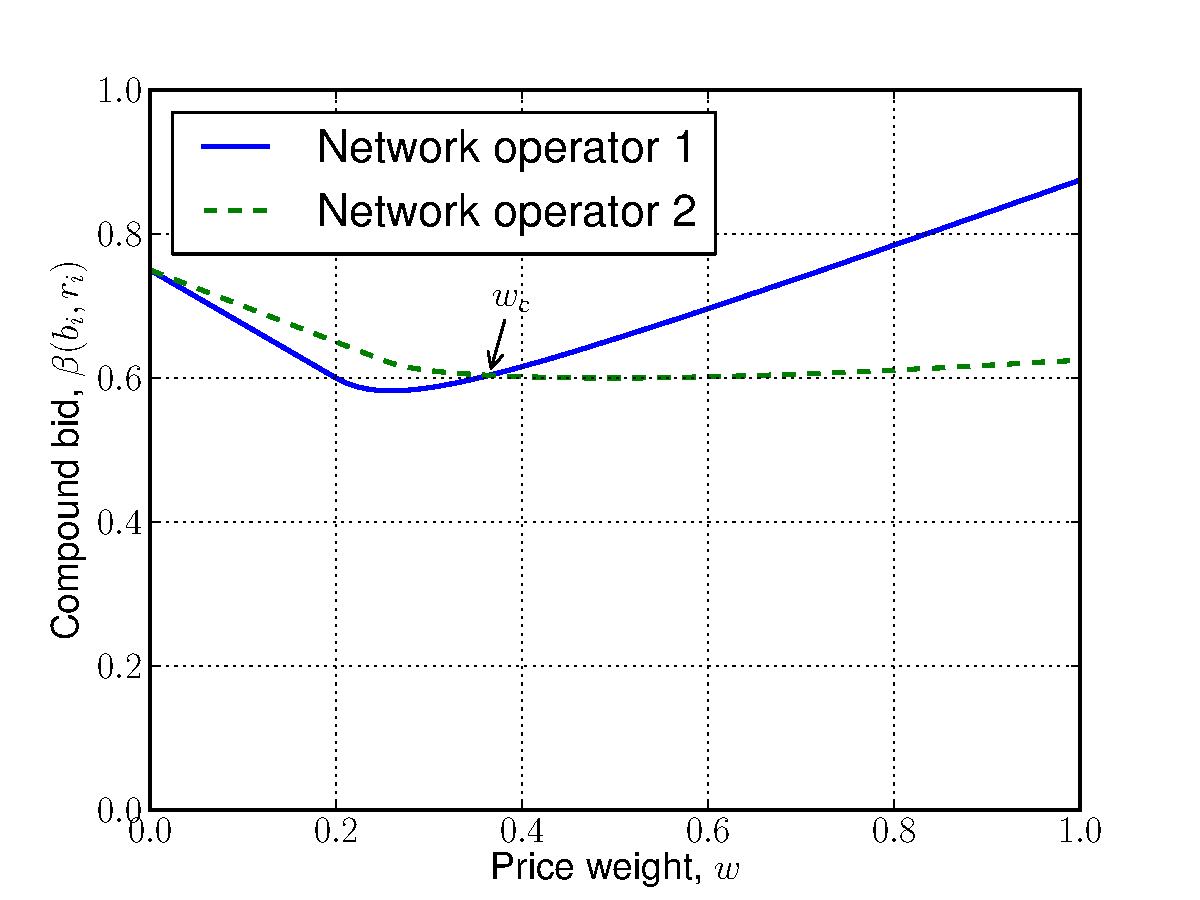
\includegraphics[width=\figsize]{Indirect/Figures/bids_restricted}
  \caption{Compound bid plotted against the price weight}
  \label{fig:bids_restricted_indirect}
  \vspace{10mm}
  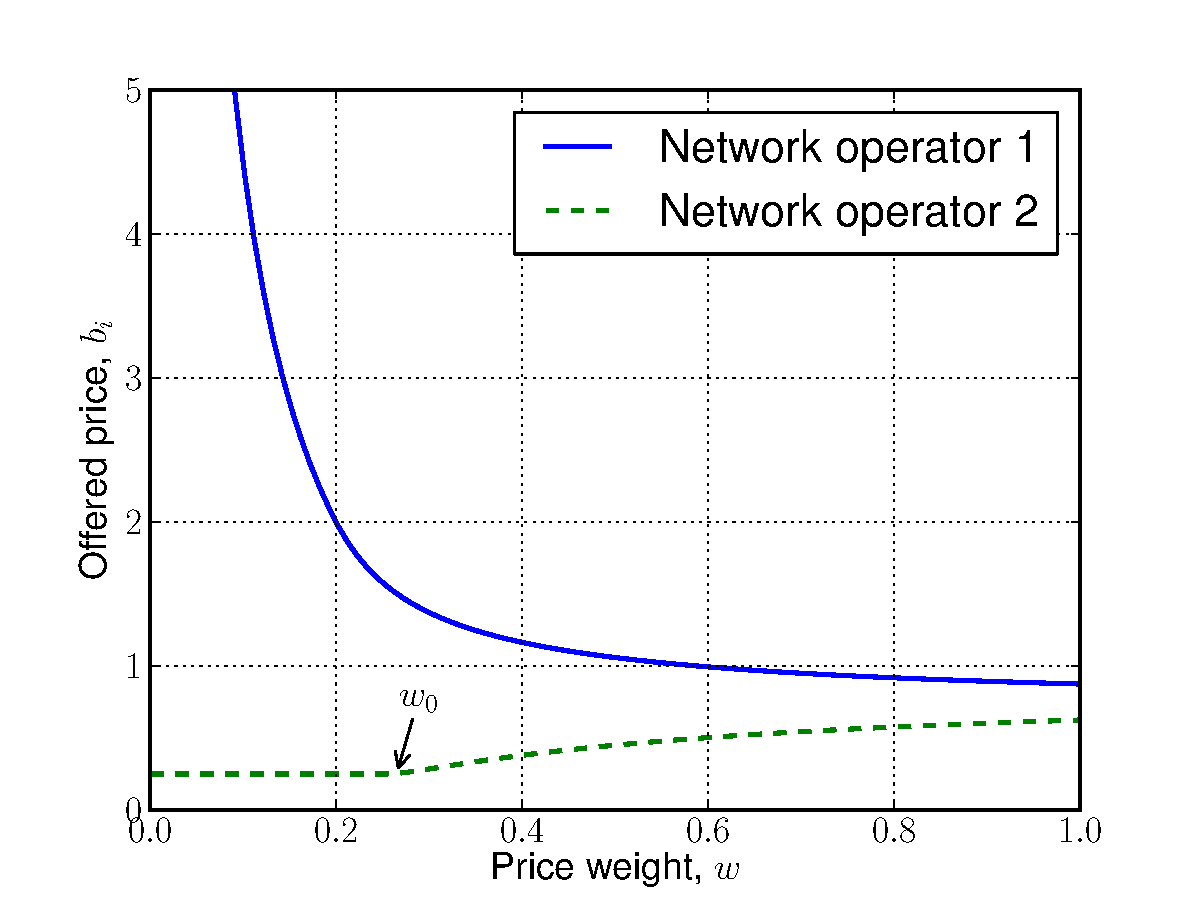
\includegraphics[width=\figsize]{Indirect/Figures/prices_restricted}
  \caption{Offered prices (bids) plotted against the price weight}
  \label{fig:prices_restricted_indirect}
\end{figure}

The result of the steps described above is the tabulation of the costs-hat and their corresponding equilibrium bids-hat for a particular price weight $w$, and reputation ratings $r_1$ and $r_2$ for both network operators, in the ranges $[\underline{\hat{c}}_1, \bar{\hat{c}}_1]$ for network operator 1 and $[\underline{\hat{c}}_2, \bar{\hat{c}}_2]$ for network operator 2.

Denote by
\begin{equation}
  \label{eq:equi_bidding_str_1_indirect}
  \hat{b}_1(\hat{c}_1) = \hat{b}_1 \quad\text{for all } \hat{c}_1\in[\underline{\hat{c}}_1, \bar{\hat{c}}_1],
\end{equation}
and
\begin{equation}
  \label{eq:equi_bidding_str_2_indirect}
  \hat{b}_2(\hat{c}_2) = \hat{b}_2 \quad\text{for all } \hat{c}_2\in[\underline{\hat{c}}_2, \bar{\hat{c}}_2]
\end{equation}
the resultant equilibrium bidding strategy functions. The problem can be transformed back into the original domain by substituting Equations~\eqref{eq:b_hat_indirect}~and~\eqref{eq:cost_hat_indirect} into Equations~\eqref{eq:equi_bidding_str_1_indirect}~and~\eqref{eq:equi_bidding_str_2_indirect}; that is,
\begin{equation*}
  \hat{b}_1(\hat{c}_1) = \hat{b}_1 \iff b_1 = \displaystyle\frac{\hat{b}_1(wc_1 + (1-w)r_1) - (1-w)r_1}{w}
\end{equation*}
for all $c_1\in[0,1]$, and
\begin{equation*}
  \hat{b}_2(\hat{c}_2) = \hat{b}_2 \iff b_2 = \displaystyle\frac{\hat{b}_2(wc_2 + (1-w)r_2) - (1-w)r_2}{w}
\end{equation*}
for all $c_2\in[0,1]$.
Keeping costs and reputation ratings fixed, one can then estimate the equilibrium bidding strategy functions with respect to the price weights by sliding the value of $w\in(0,1)$.

\begin{table}[t]
  \caption{An exemplary set of cost-reputation pairs of two network operators}
  \vspace{0.5cm}
  \begin{tabular*}{0.5\columnwidth}[L]{@{\extracolsep{\fill}}r c c}
    \hlx{vhv}
    & \textbf{Cost}, $c_i$ & \textbf{Reputation rating}, $r_i$\\
    \hlx{vhv}
    \textbf{Network operator 1} & $0.75$ & $0.25$\\
    \textbf{Network operator 2} & $0.25$ & $0.75$\\
    \hlx{vhs}
  \end{tabular*}
  \label{tab:example_restricted_indirect}
\end{table}

By way of example, the equilibrium bidding strategy functions were estimated for the set of cost-reputation pairs depicted in Table~\ref{tab:example_restricted_indirect}. Figure~\ref{fig:bids_restricted_indirect} shows the value of the compound bid, $\beta(b_i,r_i)$, for different values of $w$ for both network operators, while Figure~\ref{fig:prices_restricted_indirect} depicts the value of the monetary bid (or offered price), $b_i$, for different values of $w$ for both network operators. The numerical data in Table~\ref{tab:example_restricted_indirect} suggests that network operator 2 should be the winner for the values of $w\rightarrow 1$ since network operator 2's cost is strictly lower than that of their opponent's. On the other hand, network operator 1 should be winner for the values of $w\rightarrow 0$ since network operator 1's reputation rating is strictly lower than that of their opponent's (which implies that network operator 1's reputation is in fact strictly higher than that of their opponent's). This prediction agrees with the numerical output shown in Figure~\ref{fig:bids_restricted_indirect}. Let $w_c$ denote the value of $w$ for which an intersection between the compound bids of both network operators occurs (if it exists). In Figure~\ref{fig:bids_restricted_indirect}, $w_c\approx 0.365$. Hence, network operator 2 wins the auction for the values of $w_c < w < 1$, while network operator 1 for the values of $0 < w < w_c$.

Note, furthermore, that since we have explicitly required the network operators to bid their own costs when their probability of winning is zero, the monetary bid of network operator 2 is capped at their cost, $b_2 = 0.25$, for the values of $0 < w \le w_0$ where $w_0\approx 0.265$ (Figure~\ref{fig:prices_restricted_indirect}). In the same range of $w$, as $w$ decreases, network operator 1's bid increases in an exponential-like fashion, to finally culminate in $b_1\to\infty$ at $w=0$ in accordance with Proposition~\ref{prop:special_case_w_0_direct}. As $w\to 1$, on the other hand, the monetary bids of both network operators tend to the values specified in Proposition~\ref{prop:special_case_w_1_direct}, that is, $b_1=0.875$ and $b_2=0.625$, to finally attain those values at $w=1$.
% section restricted_case_n_2_indirect (end)

\section{Numerical Analysis} % (fold)
\label{sec:numerical_analysis_indirect}
As pointed out in Section~\ref{sec:generic_case_indirect}, the system of ODEs~\eqref{eq:foc_ode_indirect} together with the lower and upper boundary conditions~\eqref{eq:foc_ode_lower_boundary_indirect}~and~\eqref{eq:foc_ode_upper_boundary_indirect} does not possess any known closed-form solution in a generic setting, and especially when $n>2$. However, there exists a considerable research base studying methods for numerical approximation of the solution to the system of ODEs in question. See Hubbard and Paarsch~\cite{HubbardPaarsch2011} for an excellent overview of the subject.

The literature is mostly concerned with asymmetric first-price auctions in which the bidders are characterized by different probability distributions sharing a common support; that is, $F_i(\hat{c})\neq F_j(\hat{c})$ for at least one $i\in N$ such that $i\neq j, j\in N$, and for all $\hat{c}\in [\underline{\hat{c}}, \bar{\hat{c}}]$ where $[\underline{\hat{c}}, \bar{\hat{c}}] = [\underline{\hat{c}}_i, \bar{\hat{c}}_i]$ for all $i\in N$. This is not true in our case. Therefore, the methods described in Hubbard and Paarsch~\cite{HubbardPaarsch2011} have to be adapted before they can be applied to our problem.

However, both scenarios (the one considered in the literature and the one at hand) share a common difficulty: the fact that the common lower bound on bids, $\underline{\hat{b}}$, is unknown \emph{a priori} \cite{HubbardPaarsch2011}. On the other hand, since the common upper bound on bids, $\bar{\hat{b}}$, is known \emph{a priori}, it would seem that any well-known finite-difference method, such as Euler or Runge-Kutta methods, could be applied to the system of ODEs in Equation~\eqref{eq:foc_ode_indirect} with the upper bound on bids as a starting point (the so-called \emph{terminal value problem}). As shown by Hubbard and Paarsch~\cite{HubbardPaarsch2011}, the system does not satisfy the Lipschitz condition for continuity as we approach the upper bound on bids, $\bar{\hat{b}}$. Therefore, much of the theory of ordinary differential equations no longer applies. In practice, this effectively means that the numerical solution obtained using a finite-difference method applied to the terminal value problem will quickly diverge. FIX:ME Provide a graphical example.

In this section, we shall consider two numerical algorithms which overcome the aforementioned problem: the forward shooting method, and the polynomial projection method, both of which were first proposed by Bajari~\cite{Bajari2001a}. To this end, let costs, $c_i$, be drawn from a uniform distribution for all network operators as in Section~\ref{sec:restricted_case_n_2_indirect}. Again, this implies that the distribution of costs-hats, $\hat{c}_i$, is uniform with supports $[\underline{\hat{c}}_i, \bar{\hat{c}}_i] = [(1-w)r_i, (1-w)r_i + w]$ for all $i\in N$. We shall concentrate only on cases in which $J=N$; that is, $\underline{\hat{c}}_i < \bar{\hat{b}}$ for all $i\in N$. In particular, we require $w\in\left(0.5, 1\right)$ which immediately implies that $\underline{\hat{c}}_i < \bar{\hat{b}}$ for all $i\in N$ \footnote{Without loss of generality, suppose $r_1\leq\cdots\leq r_n$ with at least one inequality strict. Since $\bar{\hat{b}}\in[\bar{\hat{c}}_1, \bar{\hat{c}}_2]$ by Definition~\ref{def:upper_bound_bids_indirect}, and in particular, if $\underline{\hat{c}}_n < \bar{\hat{c}}_1$, then $\underline{\hat{c}}_n < \bar{\hat{b}}$. Thus, we require $\underline{\hat{c}}_n = (1-w)r_n < (1-w)r_1 + w = \bar{\hat{c}}_1$. This is equivalent to $1 - \frac{1}{1+r_n-r_1} < w$. Since $(r_n - r_1)\in (0, 1]$, then $1 - \frac{1}{1+r_n-r_1} \in (0,0.5]$. Therefore, if $0.5 < w$, then $1 - \frac{1}{1+r_n-r_1} < w$ for all $(r_n-r_1)\in (0,1]$.}.

Furthermore, note that assumption 3 in Assumptions~\ref{ass:assumptions_generic_indirect} is satisfied even if there exists two or more network operators characterized by the lowest reputation rating. To see this, let, without loss of generality, network operators 1 and 2 be characterized by the lowest reputation rating. Then, $\bar{\hat{c}}_1 = \bar{\hat{c}}_2$. Recall that $\bar{\hat{b}}\in [\bar{\hat{c}}_1, \bar{\hat{c}}_2]$ by Definition~\ref{def:upper_bound_bids_indirect}. Thus, $\bar{\hat{b}} = \bar{\hat{c}}_1$. For assumption 3 in Assumptions~\ref{ass:assumptions_generic_indirect} not to hold, we require $\bar{\hat{b}} = \bar{\hat{c}}_1 \leq \underline{\hat{c}}_i$ for any $i\in N$ and any $\delta>0$. But this means network operator $i$ is not a feasible bidder; that is, $i\not\in J$ by Definition~\ref{def:feasible_bidders_indirect}. A contradiction since we assumed $J = N$. Now, let $\delta = \bar{\hat{b}} - \underline{\hat{c}}_n > 0$ where $n = |N|$; that is, $r_1\leq r_n$. Then, we obtain
\begin{equation*}
(\bar{\hat{b}}-\delta, \bar{\hat{b}})\cap (\underline{\hat{c}}_i, \bar{\hat{c}}_i) = (\underline{\hat{c}}_n, \bar{\hat{b}})\cap (\underline{\hat{c}}_i, \bar{\hat{c}}_i) = (\underline{\hat{c}}_n, \bar{\hat{b}})
\end{equation*}
for all $i\in N$. The resulting set is convex, and since $(\underline{\hat{c}}_n, \bar{\hat{b}})\subset [\underline{\hat{c}}_i, \bar{\hat{c}}_i]$ for all $i\in N$, this implies that $F_i$ is strictly log-concave over $(\bar{\hat{b}}-\delta, \bar{\hat{b}})\cap (\underline{\hat{c}}_i, \bar{\hat{c}}_i)$ for all $i\in N$.

Finally, we shall concentrate on cases such that
\begin{equation*}
  \underline{\hat{c}}_i \leq \hat{c}(\underline{\hat{b}}) \quad\text{for all } i\in J.
\end{equation*}
This requirement simplifies the problem so that it is numerically tractable using (slightly modified) existing numerical methods. More specifically, it reduces the lower boundary condition in Equation~\eqref{eq:foc_ode_lower_boundary_indirect} to
\begin{equation}
  \label{eq:foc_ode_lower_boundary_reduced_indirect}
  \hat{c}_i(\underline{\hat{b}}) = \underline{\hat{c}}_i \quad\text{for all } i\in J.
\end{equation}
Without this assumption, as explained by Lebrun~\cite{Lebrun2006}, there might exist $i$ such that
\begin{equation*}
  \hat{c}(\underline{\hat{b}}) < \underline{\hat{c}}_i < \bar{\hat{b}}
\end{equation*}
which forces the bid function $\hat{b}_i$ to be extended to the interval $[\hat{c}(\underline{\hat{b}}), \bar{\hat{b}}]$, which is strictly larger than the actual support, truncated at $\bar{\hat{b}}$, $[\underline{\hat{c}}_i, \bar{\hat{b}}]$ of network operator $i$'s cost. This result is somewhat confusing since even though $F_i(\hat{c}_i) = 0$ for all $\hat{c}_i\in [\hat{c}(\underline{\hat{b}}), \underline{\hat{c}}_i]$, $\hat{b}_i(\hat{c}_i)$ is still network operator $i$'s best response for all $\hat{c}_i\in [\hat{c}(\underline{\hat{b}}), \underline{\hat{c}}_i]$. The main difficulty when considering such cases stems from the fact that for all $i\in I$, where $I = \left\{i\in J \:\middle\vert\: \hat{c}(\underline{\hat{b}}) < \underline{\hat{c}}_i < \bar{\hat{b}} \right\}$, the system of ODEs in Equation~\eqref{eq:foc_ode_indirect} reduces to
\begin{equation}
  \label{eq:foc_reduced_indirect}
  0 = \frac{1}{n'-1}\sum_{k=1}^{n'}\frac{1}{b - \hat{c}_k(b)} - \frac{1}{b - \hat{c}_i(b)}.
\end{equation}
As further explained by Lebrun~\cite{Lebrun2006}, the (inverse) equilibrium bidding functions are then determined by
\begin{equation}
  \label{eq:foc_ode_reduced_indirect}
  \frac{d}{db}\hat{c}_j(b) = \frac{1 - F_j(\hat{c}_j(b))}{f_j(\hat{c}_j(b))} \left[ \frac{1}{k(\underline{\hat{b}}) - 1}\sum_{\substack{k\in J\\ k\not\in I}}\frac{1}{b - \hat{c}_k(b)} - \frac{1}{b - \hat{c}_j(b)}\right]
\end{equation}
for network operators $j\in J, j\not\in I$, and by the system in Equation~\eqref{eq:foc_reduced_indirect} for network operators $i\in I$. Both systems are combined for all $b > \underline{\hat{b}}$ until the common function $\hat{c}_i$, $i\in I$, takes as its value the smallest lower extremity strictly smaller than $\hat{c}(\underline{\hat{b}})$. At the bid where this next smallest lower extremity is reached, the functions $\hat{c}_i$ of the network operators with this lower extremity of their supports are added to the system in Equation~\eqref{eq:foc_ode_reduced_indirect}. This process is repeated until $\hat{c}_i$ for all $i\in J$ are included in~\eqref{eq:foc_ode_reduced_indirect}. This procedure is not easily accommodated by any of the numerical methods described in the literature, or this chapter; hence, the assumption
\begin{equation*}
  \underline{\hat{c}}_i \leq \hat{c}(\underline{\hat{b}}) \quad\text{for all } i\in J.
\end{equation*}
Note, however, that this assumption cannot be enforced \emph{a priori} since $\underline{\hat{b}}$ is unknown. We can maximize the (approximate) probability of enforcing this condition reasoning as follows. Without loss of generality, suppose $r_1\leq\cdots\leq r_n$ with at least one inequality strict. If $k(\underline{\hat{b}})=n$, then, by Definition~\ref{def:lower_bound_bids_indirect}, $\underline{\hat{c}}_n\leq \hat{c}(\underline{\hat{b}})$ and $\underline{\hat{c}}_n < \underline{\hat{b}}$. Furthermore, since $\underline{\hat{b}}\in (\underline{\hat{c}}_2, \bar{\hat{b}})$, then as the distance $(\underline{\hat{c}}_n-\underline{\hat{c}}_2)\to 0$, $k(\underline{\hat{b}})\to n$. Thus, the probability that $\underline{\hat{b}}\in (\underline{\hat{c}}_n, \bar{\hat{b}})$ (assuming $\underline{\hat{b}}$ is distributed uniformly over $(\underline{\hat{c}}_2, \bar{\hat{b}})$) can be quantified as follows
\begin{equation*}
  P\left\{ \underline{\hat{b}}\in (\underline{\hat{c}}_n, \bar{\hat{b}}) \right\} = 1 - P\left\{\underline{\hat{b}}\in(\underline{\hat{c}}_2, \underline{\hat{c}}_n)\right\} = 1 - \frac{\underline{\hat{c}}_n - \underline{\hat{c}}_2}{\bar{\hat{b}}-\underline{\hat{c}}_2} = \frac{\bar{\hat{b}} - \underline{\hat{c}}_n}{\bar{\hat{b}} - \underline{\hat{c}}_2}.
\end{equation*}
In particular, for the probability of at least $0.9$, we require
\begin{equation*}
  \frac{\bar{\hat{b}} - \underline{\hat{c}}_n}{\bar{\hat{b}} - \underline{\hat{c}}_2} \geq 0.9 \iff \bar{\hat{b}}\geq 10\underline{\hat{c}}_n - 9\underline{\hat{c}}_2.
\end{equation*}
Since $\bar{\hat{c}}_1\leq \bar{\hat{b}}$ by Definition~\ref{def:upper_bound_bids_indirect}, we may write
\begin{equation*}
  \bar{\hat{c}}_1 \geq 10\underline{\hat{c}}_n - 9\underline{\hat{c}}_2 \iff w \geq 1 - \frac{1}{10r_n - 9r_2 - r_1 + 1}.
\end{equation*}
Note that, since we assumed $r_1\leq\cdots\leq r_n$ with at least inequality strict, the denominator is always strictly greater than $1$ ($10r_n - 9r_2-r_1+1 > 1$), hence guaranteeing the right-hand side of the inequality to be smaller than $1$.

To conclude, in the rest of this section, we shall concentrate on cases such that
\begin{equation*}
  w \in (0.5, 1) \quad\text{and}\quad w \geq 1 - \frac{1}{10r_n - 9r_2 - r_1 + 1}
\end{equation*}
for all $r_1,r_2,r_n\in [0,1]$ such that $r_1\leq\cdots\leq r_n$ with at least one inequality strict.

\subsection{Forward Shooting Method} % (fold)
\label{sub:forward_shooting_method_indirect}
Without loss of generality, suppose network operator 1 is characterized by the lowest reputation rating, network operator 2 by the second lowest, and so on. Hence, $\underline{\hat{c}}_1\leq \underline{\hat{c}}_2\leq \underline{\hat{c}}_i$ and $\bar{\hat{c}}_1\leq \bar{\hat{c}}_2\leq \bar{\hat{c}}_i$ for all $i\geq 2$.

The idea behind the forward shooting method is to find the best approximation of the lower bound on bids, $\underline{\hat{b}}'$ say, by successively picking a value from the feasible interval $(\underline{\hat{c}}_2, \bar{\hat{b}})$, and verifying whether a numerical solution to the initial value problem
\begin{equation}
  \label{eq:fsm_initial_value_problem_indirect}
  \begin{array}{ll}
    \displaystyle\frac{d}{db}\hat{c}_i(b) &= \displaystyle\frac{1 - F_i(\hat{c}_i(b))}{f_i(\hat{c}_i(b))}\left[ \frac{1}{n-1}\sum_{k=1}^n\frac{1}{b - \hat{c}_k(b)} - \frac{1}{b - \hat{c}_i(b)} \right] \\[2ex]
    \hat{c}_i(\underline{\hat{b}}') &= \underline{\hat{c}}_i
  \end{array}
\end{equation}
for all $i\in N$, lies within a set of permissible functions, $S_i$, such that every element of that set is a function mapping $[\underline{\hat{b}}', \bar{\hat{b}}]$ into $[\underline{\hat{c}}_i, \bar{\hat{c}}_i]$, it is monotonically increasing everywhere except possibly at $\bar{\hat{b}}$, and each function value is strictly lower than its argument except possibly at $\bar{\hat{b}}$; that is,
\begin{equation*}
  S_i\equiv\left\{s \:\middle\vert\:
  \begin{array}{l}
    s: [\underline{\hat{b}}', \bar{\hat{b}}]\to [\underline{\hat{c}}_i, \bar{\hat{c}}_i],\\
    b_1 < b_2\implies s(b_1) < s(b_2) \text{ for all }b_1,b_2\in [\underline{\hat{b}}', \bar{\hat{b}}),\\
    s(b) < b \text{ for all }b\in [\underline{\hat{b}}', \bar{\hat{b}})
  \end{array}
  \right\}.
\end{equation*}
This specification of the problem is a modified version of the First Algorithm in Bajari~\cite{Bajari2001a} (cf.~Section~3.3 in~\cite{Bajari2001a}) that accommodates for different lower and upper extremities in the supports of bidders' costs.

\begin{algorithm}
\caption{Forward shooting method}
\label{alg:forward_shooting_method}
\begin{algorithmic}
  \Require{$\epsilon\in\left(0, \bar{\hat{b}} - \underline{\hat{c}}_2\right)$}
  \Function{forwardShooting}{$low, high$}
    \State{$guess\gets 0.5\cdot(low + high)$}
    \If{$high - low < \epsilon$}
      \State\Return{$guess$}
    \Else
      \State{$bids\gets \left[guess, \bar{\hat{b}}\right)$}
      \State{$(costs_1,\dotsc,costs_n)\gets$ solve system in~\eqref{eq:fsm_initial_value_problem_indirect} with $\underline{\hat{b}}' = guess$}
      \If{$(bids,costs_i)\in S_i$ for all $i\gets \{1,\dotsc,n\}$}
        \State\Return{\Call{forwardShooting}{$low, guess$}}
      \Else
        \State\Return{\Call{forwardShooting}{$guess, high$}}
      \EndIf
    \EndIf
  \EndFunction
  \State{$low\gets \underline{\hat{c}}_2$}
  \State{$high\gets \bar{\hat{b}}$}
  \State{$\underline{\hat{b}}'\gets$ \Call{forwardShooting}{$low, high$}}
\end{algorithmic}
\end{algorithm}

The pseudo-code for the forward shooting method is depicted in listing Algorithm~\ref{alg:forward_shooting_method}. For any given tolerance, $\epsilon\in\left(0, \bar{\hat{b}} - \underline{\hat{c}}_2\right)$, the algorithm aims at finding the interval $LH\equiv[low, high]\subseteq [\underline{\hat{c}}_2, \bar{\hat{b}}]$ such that (approximately) $\underline{\hat{b}}\in LH$ and $high-low < \epsilon$. The approximation to the lower bound on bids is then found to be $\underline{\hat{b}}' = 0.5\cdot(low + high)$.

The initial guess supplied to the algorithm is the interval $[\underline{\hat{c}}_2, \bar{\hat{b}}]$. In every iteration, the guessed value for the lower bound on bids is the midpoint of the interval; that is, $guess = 0.5\cdot(low + high)$. The algorithm then uses this value as the new initial condition for the system in~\eqref{eq:fsm_initial_value_problem_indirect}. If the solution to the system lies within the set $S_i$ for all $i\in N$, then $guess$ becomes the new upper endpoint of the interval $LH$; that is, $LH = [low, guess]$. Otherwise, it becomes the new lower endpoint; that is, $LH = [guess, high]$. This procedure is repeated until the length of the interval is smaller than $\epsilon$.

In each step, the system of ODEs in~\eqref{eq:fsm_initial_value_problem_indirect} can be solved numerically using any type of finite-difference methods, such as Euler or Runge-Kutta methods. The results presented in this section were obtained using a GNU Scientific Library (GSL) implementation of the Embedded Runge-Kutta-Fehlberg (4, 5) method, provided by the Haskell package ``hmatrix'' version 0.14.1.0 \cite{GSL, HMATRIX}.

Furthermore, in the implementation of the forward shooting method, we assumed that
\begin{equation*}
  F_i(x) = \frac{x - \underline{\hat{c}}_i}{\bar{\hat{c}}_i - \underline{\hat{c}}_i} \quad\text{and}\quad f_i(x) = \frac{1}{\bar{\hat{c}}_i - \underline{\hat{c}}_i}
\end{equation*}
for all $i\in N$ and $x\in\mathbb{R}$. This assumption reduces the original initial value problem in~\eqref{eq:fsm_initial_value_problem_indirect} to
\begin{equation*}
  \begin{array}{ll}
    \displaystyle\frac{d}{db}\hat{c}_i(b) &= \displaystyle\left[ \bar{\hat{c}}_i - \hat{c}_i(b)\right]\cdot\left[ \frac{1}{n-1}\sum_{k=1}^n\frac{1}{b - \hat{c}_k(b)} - \frac{1}{b - \hat{c}_i(b)} \right], \\[2ex]
    \hat{c}_i(\underline{\hat{b}}') &= \underline{\hat{c}}_i,
  \end{array}
\end{equation*}
and it is there mainly to avoid possible divisions by zero which are not handled well by the GSL library. Situations of this type may arise due to the nature of finite-difference methods, and the fact that the system of ODEs features a fraction
\begin{equation*}
  \frac{1 - F_i(x)}{f_i(x)}
\end{equation*}
which is undefined for all $x\in\mathbb{R}$ such that $x < \underline{\hat{c}}_i$ and $x > \bar{\hat{c}}_i$ (since $f_i(x) = 0$ for all $x < \underline{\hat{c}}_i$ and $x > \bar{\hat{c}}_i$). On the other hand, by enforcing this assumption, we implicitly assume that the algorithm always operates in the feasible region; that is,
\begin{equation*}
  \hat{c}_i(b)\in [\underline{\hat{c}}_i, \bar{\hat{c}}_i] \quad\text{for all } i\in N \text{ and } b\in\left[\underline{\hat{b}}', \bar{\hat{b}}\right].
\end{equation*}
This, of course, cannot be guaranteed for all choices of $\underline{\hat{b}}'$ made by the algorithm, and therefore, it might skew the final result away from the actual value of the lower bound on bids, $\underline{\hat{b}}$.
% subsection forward_shooting_method_indirect (end)

\subsection{Polynomial Projection Method} % (fold)
\label{sub:polynomial_projection_method_indirect}

% subsection polynomial_projection_method_indirect (end)

\subsection{Other Methods} % (fold)
\label{sub:other_methods_indirect}

% subsection other_methods_indirect (end)

\subsection{Limitations} % (fold)
\label{sub:limitations_indirect}

% subsection limitations (end)
% section numerical_analysis_indirect (end)

\section{Discussion} % (fold)
\label{sec:discussion_indirect}
The aim of this section is twofold. First, the results from direct and indirect approaches are compared. Second, the prices the subscriber has to pay for each value of the price weight given a tuple of network operators' reputation ratings (in the restricted case) are examined.

\subsection{Comparison of Results from Direct and Indirect Approaches} % (fold)
\label{sub:comparison_of_results_from_direct_and_indirect_approaches_indirect}
If the network operators are assumed to submit at least their costs, then, in the restricted case, Proposition~\ref{prop:pcomp_equi_bidding_str_direct} and Conjecture~\ref{conj:pcomp_max_equi_bidding_str_direct} are ruled out by Proposition~\ref{prop:characterization_of_the_equilibrium_indirect} combined with Proposition~\ref{prop:equilibrium_restricted_indirect} since the latter establishes an analytical solution to the bidding problem while Proposition~\ref{prop:characterization_of_the_equilibrium_indirect} makes this solution unique. Furthermore, for the same reason, Proposition~\ref{prop:characterization_of_the_equilibrium_indirect} and Proposition~\ref{prop:equilibrium_restricted_indirect} prove Conjecture~\ref{conj:special_case_w_1_direct} for $n=2$ network operators and costs drawn from uniform distribution over the interval $[0,1]$ (cf. numerical example in Section~\ref{sec:restricted_case_n_2_indirect}).

However, if this assumption is relaxed, then, as showed by Kaplan and Zamir~\cite{KaplanZamir2011}, Proposition~\ref{prop:characterization_of_the_equilibrium_indirect} need no longer hold, and hence, there may exist multiple equilibria in the first-price sealed-bid auction bidding problem. As a result, both equilibria summarized in Proposition~\ref{prop:equilibrium_restricted_indirect} as well as Proposition~\ref{prop:pcomp_equi_bidding_str_direct} are valid. Kaplan and Zamir~\cite{KaplanZamir2011}, who characterize equilibria like the one specified in Proposition~\ref{prop:pcomp_equi_bidding_str_direct} as non-standard, further argue that such equilibria are important and should not be neglected.
% subsection comparison_of_results_from_direct_and_indirect_approaches (end)

\begin{figure}[p!]
  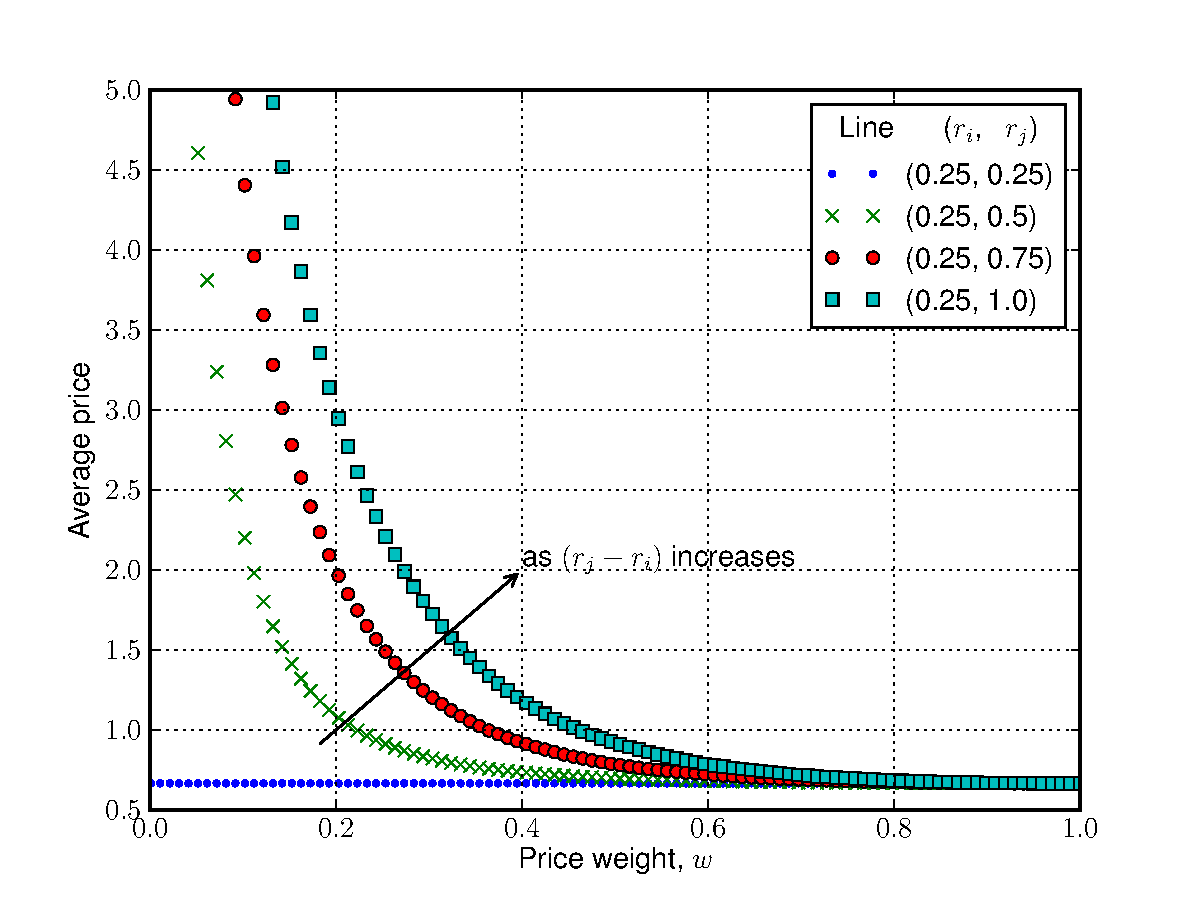
\includegraphics[width=\figsize]{Indirect/Figures/expected_prices}
  \caption{Average prices plotted against the price weight for different pairs of reputation ratings}
  \label{fig:expected_prices_indirect}
  \vspace{10mm}
  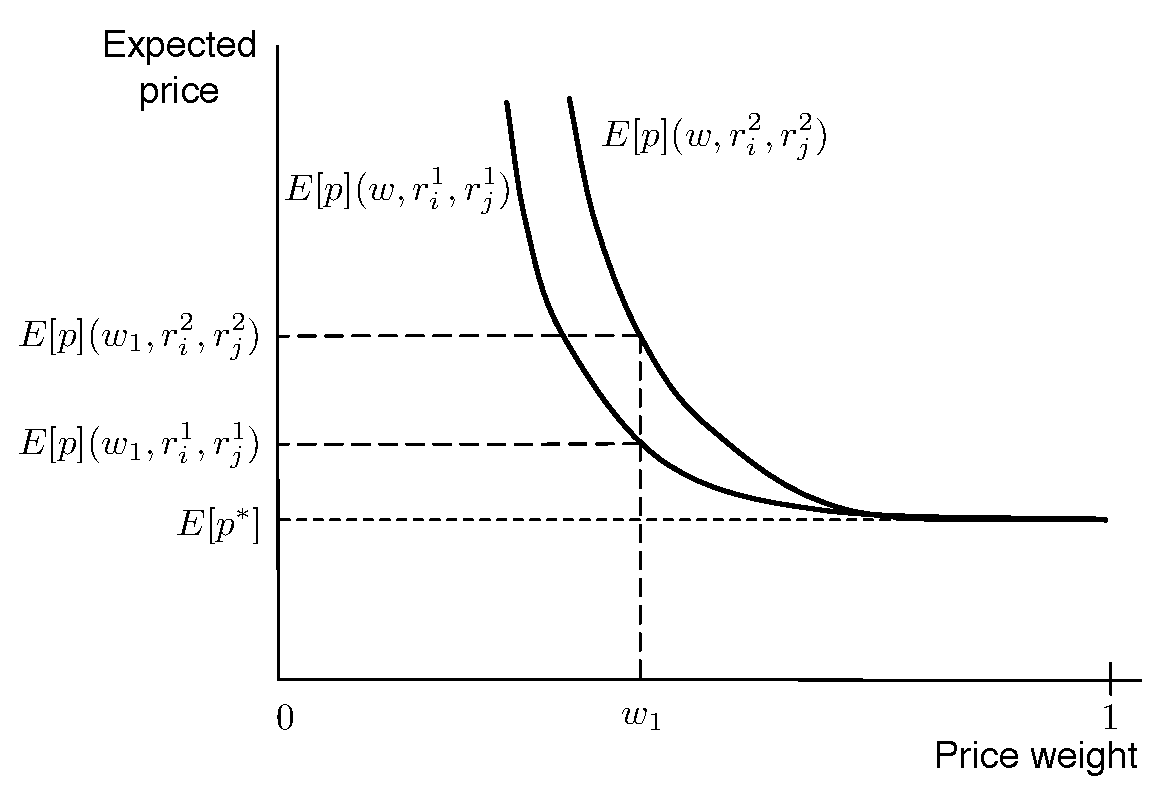
\includegraphics[width=\figsize]{Indirect/Figures/expected_prices_sensitivity}
  \caption{Sensitivity of the price weight to the expected prices}
  \label{fig:expected_prices_sensitivity_indirect}
\end{figure}

\subsection{Subscriber's Perspective: Expected Prices in Restricted Case} % (fold)
\label{sub:subscriber_s_perspective_expected_prices_in_restricted_case_indirect}
Having derived the equilibrium bidding strategy functions in the restricted case, it is possible to examine the expected prices the subscriber will have to pay for different values of the price weight given the reputation ratings of the network operators. We consider only the equilibrium bidding strategy functions in Proposition~\ref{prop:equilibrium_restricted_indirect} since they assume the network operators submit at least their costs. Hence, suppose all of the assumptions of Section~\ref{sec:restricted_case_n_2_indirect} hold; that is, there are two network operators, and costs are uniformly distributed over the interval $[0,1]$. The expected price is equivalent to the expected value of the winning bid; that is, with some abuse of notation
\begin{equation}
  \label{eq:exp_price_def_indirect}
  E[p](w,r_i,r_j) = E[b_i \:\vert\: \arg\min_{i\in N}\beta(w,b_i,r_i)],
\end{equation}
where $b_i$ is the equilibrium bid, and $\beta(w,b_i,r_i) = \beta(b_i,r_i)$ evaluated for a particular value of $w$ for all $i\in N$.

If both network operators have equal reputation ratings, $r = r_i = r_j$ say, then Corollary~\ref{cor:special_case_r_i_r_j_direct} holds for all $w\in [0,1]$. Therefore, regardless of the choice of the price weight, the subscriber expects to pay the price of
\begin{equation}
  \label{eq:exp_price_at_w_1_indirect}
  E[p^*] \equiv E[p](w,r,r) = E\left[\min_{i\in N}\frac{1+c_i}{2}\right] \quad\text{for all } w\in [0,1],
\end{equation}
which is equivalent to Equation~\eqref{eq:standard_fpa_direct} evaluated at $n=2$. In particular, for costs, $c_i$, uniformly distributed over the interval $[0,1]$, $E[p^*] = \frac{2}{3}$.

If, on the other hand, both network operators are characterized by different reputation ratings, then an analytical derivation of the expected prices for each value of the price weight given a pair of reputation ratings is cumbersome. This is due to the fact that network operators bid according to a pair of inverse equilibrium bidding functions specified in Proposition~\ref{prop:equilibrium_restricted_indirect}, which are not easily invertible. Hence, we resort to numerical methods for estimating average (sample mean) prices for selected values of the price weight given a pair of reputation ratings.

To this end, for any given pair of reputation ratings, the costs are pseudo-randomly drawn from the uniform distribution over the discretized interval $[0,1]$. For each selected price weight, the average price is averaged over 10,000 i.i.d.~observations. The Strong Law of Large Numbers (which is stated in Section~\ref{sec:probability_notation}) implies that as the number of observations tends to infinity, the average (sample mean) of the observations approaches the real mean of the distribution of the random variable in question. Therefore, an average of 10,000 observations of the price for each selected price weight should provide a reasonable approximation of the expected price for that price weight. Without loss of generality, suppose further that $r_i \le r_j$. Figure~\ref{fig:expected_prices_indirect} shows the result of the estimation for four pairs of reputation ratings: $(r_i, r_j) = (0.25, 0.25)$, $(0.25, 0.5)$, $(0.25, 0.75)$, and $(0.25, 1.0)$.

It can be observed that regardless of the values of the reputation ratings, the expected prices, $E[p](w,r_i,r_j)$, are bounded from below by $E[p^*]$ for each price weight; this is depicted in Figure~\ref{fig:expected_prices_indirect}. Hence, it can be concluded that regardless of the values of the reputation ratings, the lowest expected price is achieved for $w=1$, and will not decrease as $w$ decreases; in fact, it can only either increase or remain constant.

Furthermore, as the difference $(r_j-r_i)$ increases, the expected prices, $E[p](w,r_i,r_j)$, increase as the price weight decreases; this is depicted in Figure~\ref{fig:expected_prices_indirect}. Therefore, it can be hypothesized that the smaller the difference $(r_j-r_i)$, the less (expected) price sensitive the price weight; that is, for any $w_1\in[0,1]$, if $(r^2_j-r^2_i) > (r^1_j-r^1_i)$ for all $r^1_i,r^1_j,r^2_i,r^2_j\in [0,1]$, then $E[p](w_1,r^2_i,r^2_j) \ge E[p](w_1,r^1_i,r^1_j)$ (Figure~\ref{fig:expected_prices_sensitivity_indirect}). In other words, for any expected price, as the difference $(r_j-r_i)$ between the reputation ratings of the network operators increases, the price weight has to increase (or remain constant) in order to keep the expected price fixed.
% subsection subscriber_s_perspective_expected_prices_in_restricted_case (end)
% section discussion (end)

\section{Summary}
\label{sec:summary_indirect}

\section{Proofs}
\label{sec:proofs_indirect}
\begin{proof}[Proof of Proposition~\ref{prop:regularity_conditions_indirect}]
Proof of 1) is trivial. To prove 2) and 3), we note that for all $x\in [(1-w)r_i, (1-w)r_i + w]$,
\begin{align*}
  F_i(x)
  &= P\{\hat{C}_i\le x\} \\
  &= P\{wC + (1-w)r_i\le x\} \\
  &= P\left\{ C\le \frac{x - (1-w)r_i}{w} \right\}
\end{align*}
since $\hat{c}_i = wc_i + (1-w)r_i$ and $w\neq 0$. Hence,
\begin{equation*}
  F_i(x) = F_C\left( \frac{x - (1-w)r_i}{w} \right)
\end{equation*}
and
\begin{equation*}
  \frac{x - (1-w)r_i}{w}\in [0,1]
\end{equation*}
for all $x\in [(1-w)r_i, (1-w)r_i + w]$. Therefore, since $F_C$ is differentiable over $(0,1]$ with a derivative $f_C$ locally bounded away from zero over this interval, by extension, $F_i$ is differentiable over $((1-w)r_i, (1-w)r_i + w]$ with a derivative $f_i$ locally bounded away from zero over this interval, and this proves 2). Moreover, since $F_C$ is atomless, by extension, $F_i$ is atomless, and this proves 3).
\end{proof}

\begin{proof}[Proof of Proposition~\ref{prop:characterization_of_the_equilibrium_indirect}]
To prove existence, we note that Lebrun~\cite{Lebrun2006} proves the existence of a pure-strategy Bayesian Nash equilibrium where network operators submit at least their costs-hat (cf. C.5 Characterization with Possibly Different Lower and Upper Extremities in~\cite{Lebrun2006}).

To prove uniqueness, without loss of generality, let network operator 1 be characterized by the lowest reputation rating, network operator 2 by the second lowest, and so on; that is, let $r_1 \leq r_2 \leq\cdots \leq r_n$. This implies $\underline{\hat{c}}_1 \leq \underline{\hat{c}}_2 \leq\cdots \leq \underline{\hat{c}}_n$ and $\bar{\hat{c}}_1 \leq \bar{\hat{c}}_2 \leq \cdots\leq \bar{\hat{c}}_n$. Since Assumptions~\ref{ass:assumptions_generic_indirect} are satisfied, then at least one inequality is strict. We need to consider two cases: 1) $r_1 < r_2$, and 2) $r_1 = r_2$. When 1) holds, then $\bar{\hat{c}}_1 < \bar{\hat{c}}_2$, implying that the additional condition (ii) in Theorem~1 in Lebrun~\cite{Lebrun2006} holds. Otherwise, if 2) holds, then the additional condition (iii) in Theorem~1 in Lebrun~\cite{Lebrun2006} is satisfied. Thus, the considered first-price auction has one and only one pure-strategy Bayesian Nash equilibrium where network operators bid at least their costs-hat.
\end{proof}

\begin{proof}[Proof of Proposition~\ref{prop:equilibrium_restricted_indirect}]
The proof is analogous to the proof of Proposition~1 in Kaplan and Zamir~\cite{KaplanZamir2007}.
\end{proof}
